% This file was created with tikzplotlib v0.10.1.
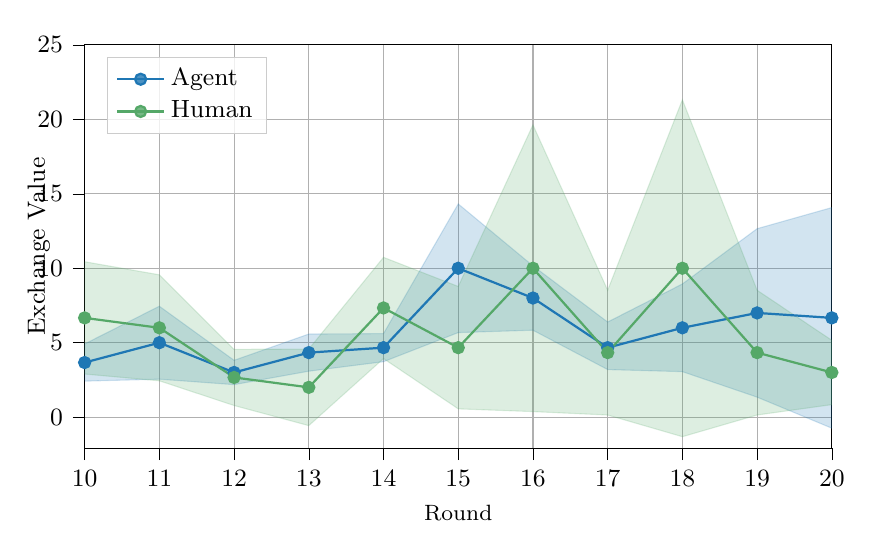
\begin{tikzpicture}

\definecolor{darkgrey176}{RGB}{176,176,176}
\definecolor{forestgreen4416044}{RGB}{85,168,104}
\definecolor{lightgrey204}{RGB}{204,204,204}
\definecolor{steelblue31119180}{RGB}{31,119,180}
% \begin{axis}[
% legend cell align={left},
% legend style={
%   fill opacity=0.8,
%   draw opacity=1,
%   text opacity=1,
%   at={(0.03,0.97)},
%   anchor=north west,
%   draw=lightgrey204
% },
% tick align=outside,
% tick pos=left,
% x grid style={darkgrey176},
% xlabel={Turn},
% xmajorgrids,
% xmin=9.5, xmax=20.5,
% xtick style={color=black},
% y grid style={darkgrey176},
% ylabel={Trade Volume},
% ymajorgrids,
% ymin=-2.44507934888324, ymax=22.4450793488832,
% ytick style={color=black}
% ]
\begin{axis}[
scale=0.9,           
width=1\textwidth,  % 减半宽度
height=0.6\textwidth,
legend cell align={left},
legend style={
  fill opacity=0.8,
  draw opacity=1,
  text opacity=1,
  at={(0.03,0.97)},
  anchor=north west,
  draw=lightgrey204,
    font=\small
},
tick align=outside,
tick pos=left,
x grid style={darkgrey176},
tick label style={font=\small},
xlabel=Round,
xlabel style={font=\footnotesize},
xmajorgrids,
xmin=10, xmax=20,    % 保持原始坐标范围
xtick style={color=black},
y grid style={darkgrey176},
ylabel={Exchange Value},
ylabel style={
    inner sep=0pt,    
    yshift=-8pt,
    font=\small
},
ymajorgrids,
ymin=-2.1, ymax=25,
ytick style={color=black}
]


% \path [draw=forestgreen4416044, fill=forestgreen4416044, opacity=0.2]
% (axis cs:10,10.4379028329949)
% --(axis cs:10,2.89543050033841)
% --(axis cs:11,2.44097391598956)
% --(axis cs:12,0.78104858350254)
% --(axis cs:13,-0.57)
% --(axis cs:14,3.93398699093814)
% --(axis cs:15,0.557057331354016)
% --(axis cs:16,0.373647281204232)
% --(axis cs:17,0.143398303341154)
% --(axis cs:18,-1.31370849898476)
% --(axis cs:19,0.143398303341154)
% --(axis cs:20,0.839753100530713)
% --(axis cs:20,5.16024689946929)
% --(axis cs:20,5.16024689946929)
% --(axis cs:19,8.52326836332551)
% --(axis cs:18,21.3137084989848)
% --(axis cs:17,8.52326836332551)
% --(axis cs:16,19.6263527187958)
% --(axis cs:15,8.77627600197932)
% --(axis cs:14,10.7326796757285)
% --(axis cs:13,4.57)
% --(axis cs:12,4.55228474983079)
% --(axis cs:11,9.55902608401044)
% --(axis cs:10,10.4379028329949)
% --cycle;
% \addlegendimage{area legend, draw=forestgreen4416044, fill=forestgreen4416044, opacity=0.2}
% \addlegendentry{Std}

% \addplot [thick, forestgreen4416044, mark=*, mark size=2, mark options={solid}]
% table {%
% 10 6.66666666666667
% 11 6
% 12 2.66666666666667
% 13 2
% 14 7.33333333333333
% 15 4.66666666666667
% 16 10
% 17 4.33333333333333
% 18 10
% 19 4.33333333333333
% 20 3
% };
% \addlegendentry{Mean}





\path [draw=steelblue31119180, fill=steelblue31119180, opacity=0.2]
(axis cs:10,4.91388579559131)
--(axis cs:10,2.41944753774202)
--(axis cs:11,2.55051025721682)
--(axis cs:12,2.18350341907227)
--(axis cs:13,3.08611420440869)
--(axis cs:14,3.7238576250846)
--(axis cs:15,5.67950620106143)
--(axis cs:16,5.83975310053071)
--(axis cs:17,3.19526214587564)
--(axis cs:18,3.05607971122405)
--(axis cs:19,1.34314575050762)
--(axis cs:20,-0.742036923630955)
--(axis cs:20,14.0753702569643)
--(axis cs:20,14.0753702569643)
--(axis cs:19,12.6568542494924)
--(axis cs:18,8.94392028877595)
--(axis cs:17,6.3880711874577)
--(axis cs:16,10.1602468994693)
--(axis cs:15,14.3204937989386)
--(axis cs:14,5.60947570824873)
--(axis cs:13,5.58055246225798)
--(axis cs:12,3.81649658092773)
--(axis cs:11,7.44948974278318)
--(axis cs:10,4.91388579559131)
--cycle;
% \addlegendimage{area legend, draw=steelblue31119180, fill=steelblue31119180, opacity=0.2}
% \addlegendentry{Breach Std}

\path [draw=forestgreen4416044, fill=forestgreen4416044, opacity=0.2]
(axis cs:10,10.4379028329949)
--(axis cs:10,2.89543050033841)
--(axis cs:11,2.44097391598956)
--(axis cs:12,0.78104858350254)
--(axis cs:13,-0.57)
--(axis cs:14,3.93398699093814)
--(axis cs:15,0.557057331354016)
--(axis cs:16,0.373647281204232)
--(axis cs:17,0.143398303341154)
--(axis cs:18,-1.31370849898476)
--(axis cs:19,0.143398303341154)
--(axis cs:20,0.839753100530713)
--(axis cs:20,5.16024689946929)
--(axis cs:20,5.16024689946929)
--(axis cs:19,8.52326836332551)
--(axis cs:18,21.3137084989848)
--(axis cs:17,8.52326836332551)
--(axis cs:16,19.6263527187958)
--(axis cs:15,8.77627600197932)
--(axis cs:14,10.7326796757285)
--(axis cs:13,4.57)
--(axis cs:12,4.55228474983079)
--(axis cs:11,9.55902608401044)
--(axis cs:10,10.4379028329949)
--cycle;
% \addlegendimage{area legend, draw=forestgreen4416044, fill=forestgreen4416044, opacity=0.2}
% \addlegendentry{Human Std}

\addplot [thick, steelblue31119180, mark=*, mark size=2, mark options={solid}]
table {%
10 3.66666666666667
11 5
12 3
13 4.33333333333333
14 4.66666666666667
15 10
16 8
17 4.66666666666667
18 6
19 7
20 6.66666666666667
};
\addlegendentry{Agent}
\addplot [thick, forestgreen4416044, mark=*, mark size=2, mark options={solid}]
table {%
10 6.66666666666667
11 6
12 2.66666666666667
13 2
14 7.33333333333333
15 4.66666666666667
16 10
17 4.33333333333333
18 10
19 4.33333333333333
20 3
};
\addlegendentry{Human}





\end{axis}

\end{tikzpicture}
